\documentclass[border=0pt]{standalone}
\usepackage{fontspec}
\setmainfont{Carlito}
\usepackage{unicode-math}
\setmathfont{Latin Modern Math}
\usepackage{xcolor}
\usepackage{booktabs}
\usepackage{tikz}
\usepackage{graphicx}

\definecolor{canvabg}{RGB}{246,244,241}
\definecolor{textDark}{RGB}{40,40,40}
\definecolor{textMute}{RGB}{125,120,113}
\definecolor{accent}{RGB}{18,125,108}
\definecolor{trough}{RGB}{160,55,50}
\definecolor{bridge}{RGB}{30,90,140}

\pagecolor{canvabg}

\providecommand{\Cref}[1]{}
\providecommand{\cref}[1]{}
\providecommand{\ab}[1]{#1}

\renewcommand{\arraystretch}{1.35}

\begin{document}
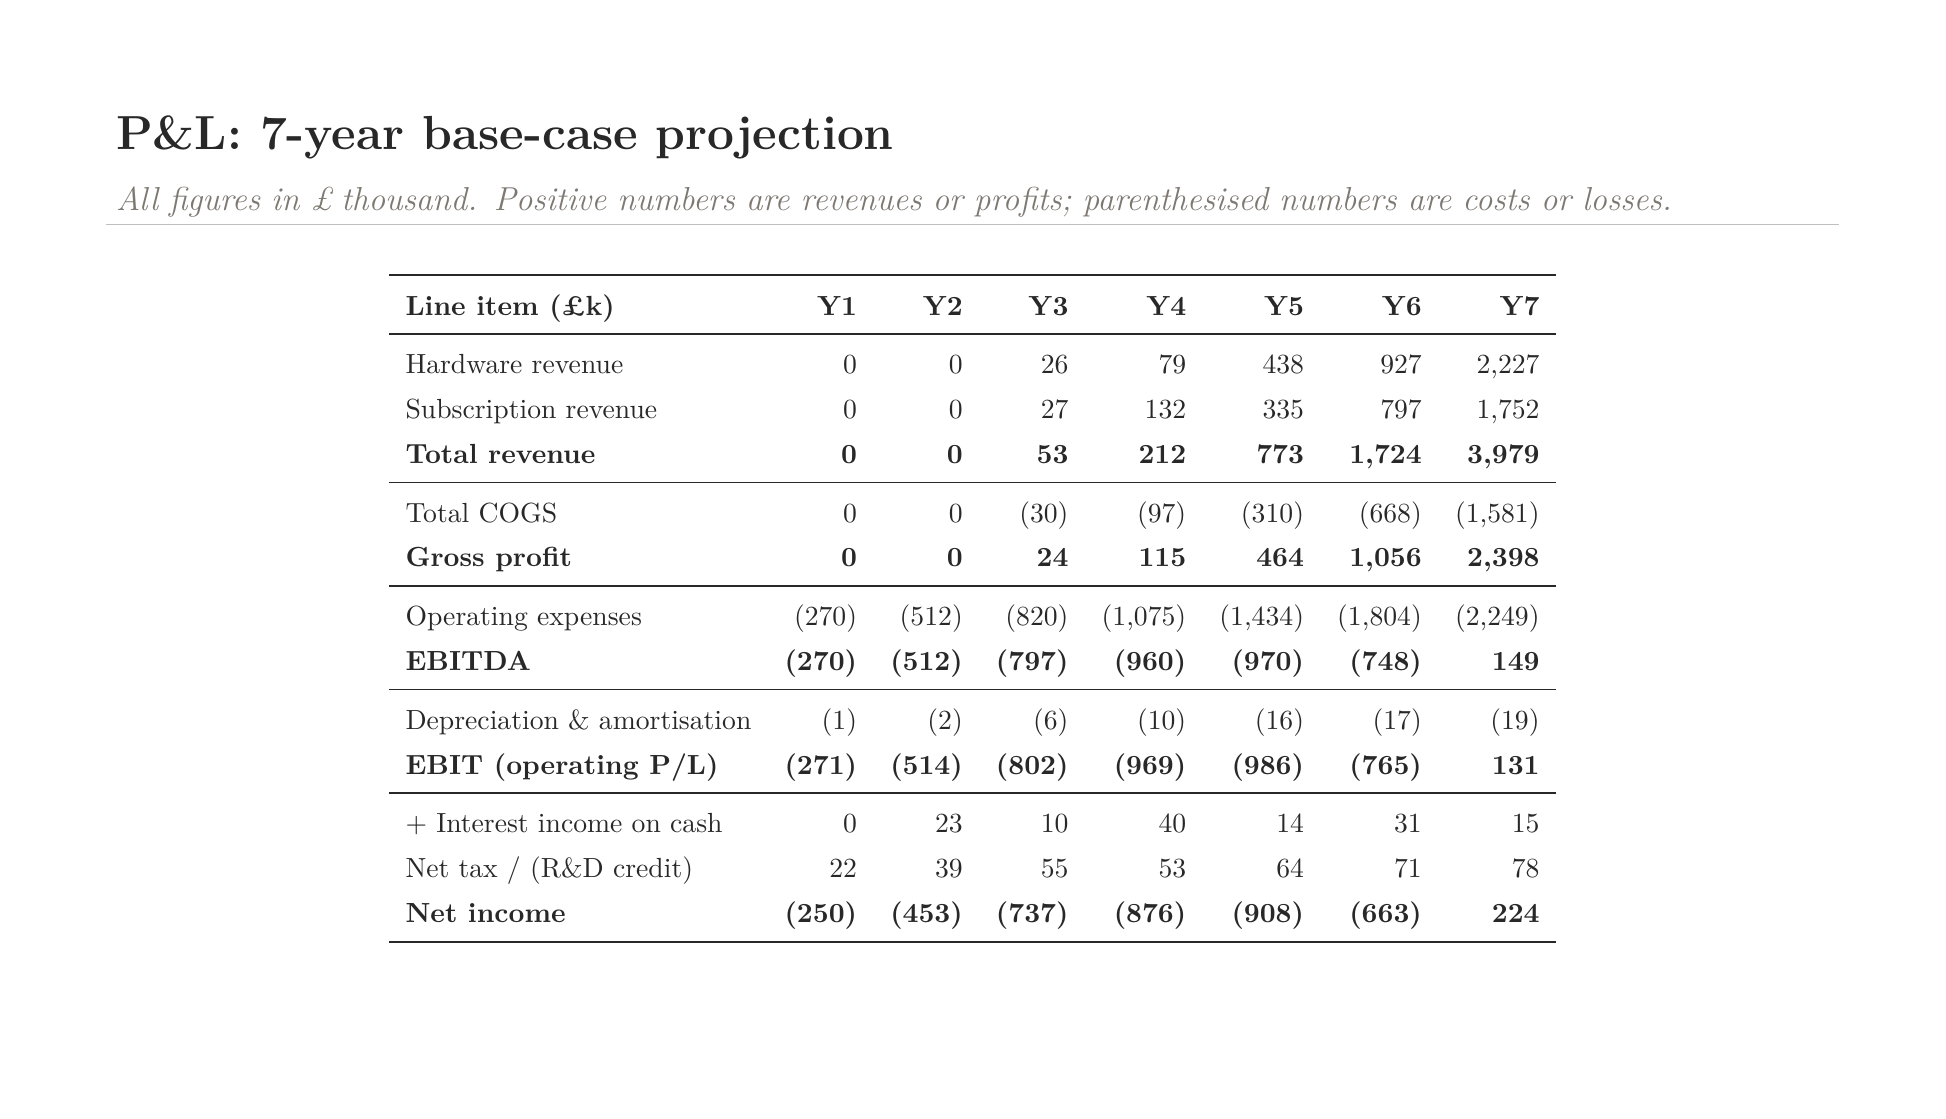
\begin{tikzpicture}[every node/.style={text=textDark}]
\useasboundingbox (0,0) rectangle (24, 13.5);

\node[anchor=north west, font=\bfseries\LARGE] at (1.0, 12.5)
    {P\&L: 7-year base-case projection};
\node[anchor=north west, font=\itshape\large, text=textMute, text width=22cm]
    at (1.0, 11.6)
    {All figures in \pounds{}\,thousand. Positive numbers are revenues or
     profits; parenthesised numbers are costs or losses.};

\draw[gray!50, line width=0.5pt] (1.0, 11.0) -- (23.0, 11.0);

\node[anchor=north, font=\normalsize] at (12.0, 10.5) {%
\begin{tabular}{lrrrrrrr}
    \toprule
    \textbf{Line item (\pounds k)} & \textbf{Y1} & \textbf{Y2} & \textbf{Y3} & \textbf{Y4} & \textbf{Y5} & \textbf{Y6} & \textbf{Y7} \\
    \midrule
    Hardware revenue                     & 0     & 0      & 26    & 79     & 438    & 927     & 2{,}227 \\
    Subscription revenue                 & 0     & 0      & 27    & 132    & 335    & 797     & 1{,}752 \\
    \textbf{Total revenue}             & \textbf{0}     & \textbf{0}     & \textbf{53}    & \textbf{212}   & \textbf{773}   & \textbf{1{,}724} & \textbf{3{,}979} \\
    \midrule
    Total COGS                           & 0     & 0      & (30)  & (97)   & (310)  & (668)   & (1{,}581) \\
    \textbf{Gross profit}              & \textbf{0}     & \textbf{0}     & \textbf{24}    & \textbf{115}   & \textbf{464}   & \textbf{1{,}056} & \textbf{2{,}398} \\
    \midrule
    Operating expenses                   & (270) & (512)  & (820) & (1{,}075) & (1{,}434) & (1{,}804) & (2{,}249) \\
    \textbf{EBITDA}                    & \textbf{(270)} & \textbf{(512)} & \textbf{(797)} & \textbf{(960)} & \textbf{(970)} & \textbf{(748)} & \textbf{149} \\
    \midrule
    Depreciation \& amortisation         & (1)   & (2)    & (6)   & (10)   & (16)   & (17)    & (19) \\
    \textbf{EBIT (operating P/L)}      & \textbf{(271)} & \textbf{(514)} & \textbf{(802)} & \textbf{(969)} & \textbf{(986)} & \textbf{(765)} & \textbf{131} \\
    \midrule
    + Interest income on cash            & 0     & 23     & 10    & 40     & 14     & 31      & 15 \\
    Net tax / (R\&D credit)              & 22    & 39     & 55    & 53     & 64     & 71      & 78 \\
    \textbf{Net income}                & \textbf{(250)} & \textbf{(453)} & \textbf{(737)} & \textbf{(876)} & \textbf{(908)} & \textbf{(663)} & \textbf{224} \\
    \bottomrule
\end{tabular}
};

\end{tikzpicture}
\end{document}
